\documentclass{article}
\usepackage{jheppub,physics,amsfonts,graphicx,tensor,cleveref}
\usepackage[export]{adjustbox}
\newcommand{\ii}{\mathrm{i}}
\newcommand{\me}{\mathrm{e}}
\newcommand{\cd}{\mathcal{D}}
\DeclareMathOperator{\arcsinh}{arcsinh}
\counterwithout{equation}{section}


\title{Homework 1}
\author{Shangjie Zhou}
\emailAdd{ZhouShangjie@purdue.edu}
\toccontinuoustrue
\notoc


\begin{document}

\maketitle


\section*{Problem 1}
\subsection*{(i)}
For simplicity, we consider the case of swapping the $\alpha$-th and $\beta$-th electrons where $\alpha<\beta$.
The term $\exp(-\sum_{i=1}^Nz_i \bar{z}_i/4l^2)$ is obviously symmetric under $\alpha\leftrightarrow \beta$.
We only need to consider the terms involving $z_\alpha$ and $z_\beta$ in $\prod_{i<j}(z_i-z_j)^p$, which are listed below:

\begin{equation}\label{eq:terms_1}
    \prod_{j>\beta}(z_\alpha-z_j)^p\prod_{j>\beta}(z_\beta-z_j)^p
\end{equation}


\begin{equation}\label{eq:terms_2}
    \prod_{i<\alpha}(z_i-z_\alpha)^p\prod_{i<\beta}(z_i-z_\beta)^p
\end{equation}

\begin{equation}\label{eq:terms_3}
    \prod_{\beta>i>\alpha}(z_\beta-z_i)^p\prod_{\beta>i>\alpha}(z_i-z_\alpha)^p
\end{equation}

\begin{equation}\label{eq:terms_4}
    (z_\beta-z_\alpha)^p
\end{equation}
After swapping $\alpha$ and $\beta$, we can see that \cref{eq:terms_1,eq:terms_2,eq:terms_3} are all symmetric, while \cref{eq:terms_4} changes sign.
Therefore, the whole wave function changes sign after swapping two electrons, which means that the wave function is antisymmetric.

If $p$ is even, the wave function will be symmetric after swapping.
In addition, it has translastion symmetry, rotation symmetry and reflection symmetry.
\subsection*{(ii)}
When $p=1$, the Laughlin wave function becomes
\begin{equation}
    \Psi(z_1,z_2,\ldots,z_N)=\prod_{i<j}(z_i-z_j)\exp\left(-\sum_{i=1}^Nz_i \bar{z}_i/4l^2\right)
\end{equation}
and it can be written as a Slater determinant:
\begin{equation}
    \Psi(z_1,z_2,\ldots,z_N)\sim\begin{vmatrix}
        \psi_{0,0}(z_1) & \psi_{0,0}(z_2) & \cdots & \psi_{0,0}(z_N)\\
        \psi_{0,1}(z_1) & \psi_{0,1}(z_2) & \cdots & \psi_{0,1}(z_N)\\
        \vdots & \vdots & \ddots & \vdots\\
        \psi_{0,N-1}(z_1) & \psi_{0,N-1}(z_2) & \cdots & \psi_{0,N-1}(z_N)
    \end{vmatrix}
\end{equation}
where $\psi_{0,m}(z)=\frac{1}{\sqrt{2\pi 2^m m! l^{2}}}\left(\frac{z}{l}\right)^m\exp(-|z|^2/4l^2)$ is the single-particle wave function in the lowest Landau level with angular momentum $m$.

\vfill

\subsection*{(iii)}
When $p=3$ and $N=2$, the Laughlin wave function is
\begin{equation}
    \Psi(z_1,z_2)=(z_1-z_2)^3\exp\left(-\frac{|z_1|^2+|z_2|^2}{4l^2}\right)
\end{equation}
We can expand the polynomial part:
\begin{equation}
    (z_1-z_2)^3=z_1^3-3z_1^2z_2+3z_1z_2^2-z_2^3
\end{equation}
If we are only allowed to use one Slater determinant, the only possible choice is
\begin{equation}
    \Psi(z_1,z_2)=\frac{1}{\sqrt{2!}}\begin{vmatrix}
        \psi_{0,a}(z_1) & \psi_{0,a}(z_2)\\
        \psi_{0,b}(z_1) & \psi_{0,b}(z_2)
    \end{vmatrix}=\frac{1}{\sqrt{2}}(\psi_{0,0}(z_1)\psi_{0,1}(z_2)-\psi_{0,1}(z_1)\psi_{0,0}(z_2))
\end{equation}
where $a,b=0,1,2,3$ and $a\neq b$.
However, it is not possible to find $a$ and $b$ such that the polynomial part matches $(z_1-z_2)^3$.
Therefore, we need more than one Slater determinant to represent the Laughlin wave function.

\subsection*{(iv)}
When $N=3$, the polynomial part of the Laughlin wave function is
\begin{equation}
    (z_1-z_2)^3(z_2-z_3)^3(z_3-z_1)^3
\end{equation}
Notice that the polynomial part of a single Slater determinant has the following form (up to a normalization factor):
\begin{equation}
    \begin{vmatrix}
        z_1^{a} & z_2^{a} & z_3^{a}\\
        z_1^{b} & z_2^{b} & z_3^{b}\\
        z_1^{c} & z_2^{c} & z_3^{c}
    \end{vmatrix}
\end{equation}
and it contains only monomials like $z_1^{a}z_2^{b}z_3^{c}$ where $a,b,c$ are all different.
Therefore, in order to find the number of Slater determinants needed to represent the Laughlin wave function, we need to count the number of different monomials in the expansion of $(z_1-z_2)^3(z_2-z_3)^3(z_3-z_1)^3$ where the powers of $z_1,z_2,z_3$ are all different.
After expanding the polynomial, there are 5 kind of such monomials and we write it as $(a,b,c)$ which is an unordered triplet representing the powers of $z_1,z_2,z_3$:
\begin{equation}
    (0,3,6), (0,4,5), (1,2,6), (1,3,5), (2,3,4)
\end{equation}
Therefore, we need 5 Slater determinants to represent the Laughlin wave function.

\section*{Problem 2}
For simplicity, we work with periodic boundary condition with period $L$, so there are $N=L/a$ lattice sites.
Since there is a displacement $u$ for each site, the new lattice constant is $2a$, which will change the Brillouin zone.
\subsection*{(i)}
The total energy for the negative energy levels is
\begin{equation}
    \begin{split}
        E(u)&=-\frac{L}{2\pi}\int_{-\pi/2a}^{\pi/2a}\epsilon_k \dd{k}=-\frac{L}{2\pi}\int_{-\pi/2a}^{\pi/2a} \dd{k}\sqrt{\frac{v^2}{a^2}\cos[2](ka)+\Delta^2}\\
            &=-\frac{L}{2\pi}\int_{-\pi/2a}^{\pi/2a}\dd{p}\sqrt{\frac{v^2}{a^2}\sin[2](ap)+\Delta^2}\\
            &=-\frac{L\Delta}{\pi a}\int_0^{\pi/2}\dd{x}\sqrt{1+\frac{v^2}{a^2\Delta^2}\sin[2](x)}\\
            &=-\frac{L\Delta}{\pi a}E\left(-\frac{v^2}{a^2\Delta^2}\right)
    \end{split}
\end{equation}
where $E(m)=\int_0^{\pi/2}\dd{x}\sqrt{1-m\sin[2](x)}$ is the complete elliptic integral of the second kind.


\subsection*{(ii)}
When $\Delta\ll t_0$, we have $-v^2/a^2\Delta^2\gg 1$, and we can use the asymptotic form of $E(m)$ when $m\to -\infty$:
\begin{equation}
    E(m)=\sqrt{-m}+\frac{1}{4\sqrt{-m}}\left(\ln(-16m)-1\right)
\end{equation}
Therefore, we have 
\begin{equation}
    E(u)=-\frac{Lv}{\pi a^2}-\frac{\Delta^2 La}{4\pi v}\left(\ln\left(\frac{16v^2}{a^2\Delta^2}\right)-1\right)
\end{equation}

\subsection*{(iii)}
If we use the approximated form of $\epsilon_p\approx\tilde{\epsilon}_p=\pm\sqrt{v^2 p^2+\Delta^2}$, the total energy for the negative energy levels is
\begin{equation}
    \begin{split}
        \tilde{E}(u)&=-\frac{L}{2\pi}\int_{-\pi/2a}^{\pi/2a}\dd{p}\sqrt{v^2 p^2+\Delta^2}\\
                    &=\frac{L}{2\pi}\eval{\frac{pv\sqrt{p^2 v^2+\Delta^2}+\Delta^2\arcsinh(\frac{pv}{\Delta})}{2v}}_{-\pi/2a}^{\pi/2a}\\
                    &=\frac{\pi L\sqrt{\pi^2 v^2+4\Delta^2 a^2}}{8\pi a^2}+\frac{\Delta^2 L}{2\pi v}\arcsinh(\frac{\pi v}{2a\Delta})
    \end{split}
\end{equation}
\begin{center}
    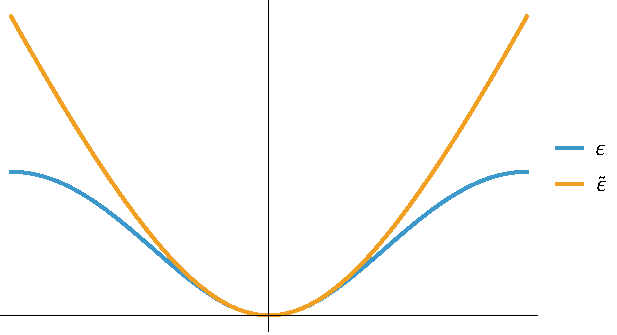
\includegraphics[width=0.5\textwidth]{plot/plot1.pdf}
\end{center}

\subsection*{(iv)}
The total energy is the sum of electron energy and elastic energy:
\begin{subequations}
    \begin{align}
        E_{tot}(u)&=E(u)+E_{el}(u)= -\frac{L\Delta}{\pi a}E\left(-\frac{v^2}{a^2\Delta^2}\right)+\frac{L\kappa u^2}{2a}\\
    \tilde{E}_{tot}(u)&=\tilde{E}(u)+E_{el}(u)= \frac{\pi L\sqrt{\pi^2 v^2+4\Delta^2 a^2}}{8\pi a^2}+\frac{\Delta^2 L}{2\pi v}\arcsinh(\frac{\pi v}{2a\Delta})+\frac{L\kappa u^2}{2a}
    \end{align}
\end{subequations}
If we want to minimize the total energy, we need to set $\pdv{E_{tot}}{u}=0$ or $\pdv{\tilde{E}_{tot}}{u}=0$.



\subsection*{(v)}
Since there are two bands, the partition function of noninteracting fermions is
\begin{equation}
    Z=\prod_k(1+\me^{-\epsilon_k/T})(1+\me^{\epsilon_k/T})
\end{equation}
To compute the free energy, we have 
\begin{equation}
    \begin{split}
        F(\Delta)&=-T\log Z\\
                 &=-T\sum_k\log((1+\me^{-\epsilon_k/T})(1+\me^{\epsilon_k/T}))\\
                 &=-T\sum_k\log(2+2\cosh(\epsilon_k/T))\\
                 &=-T\sum_k\log(4\cosh[2](\epsilon_k/2T))\\
                 &=-T\int_{-\pi/2a}^{\pi/2a}\frac{L\dd{p}}{2\pi}\log(4\cosh[2](\epsilon_p/2T))\\
                 &=-T\log(4)\frac{L}{a}-2T\int_{-\pi/2a}^{\pi/2a}\frac{L\dd{p}}{2\pi}\log(\cosh(\frac{1}{2T}\sqrt{\frac{v^2}{a^2}\sin[2](ap)+\Delta^2}))\\
    \end{split}
\end{equation}


\subsection*{(vi)}
The elastic energy is 
\begin{equation}
    E_{el}=N\frac{\kappa u^2}{2}=\frac{L\kappa u^2}{2a}
\end{equation}
where $\kappa$ is the elastic constant.
After using $\Delta=2\alpha\abs{u}$, we have 
\begin{equation}
    E_{el}=\frac{L\kappa a\Delta^2}{8\alpha^2}
\end{equation}

\subsection*{(vii)}
The energy that we need to minimize is
\begin{equation}
    E_{tot}(\Delta)=F(\Delta)+E_{el}(\Delta)= -T\log(4)\frac{L}{a}-2T\int_{-\pi/2a}^{\pi/2a}\frac{L\dd{p}}{2\pi}\log(\cosh(\frac{1}{2T}\sqrt{\frac{v^2}{a^2}\sin[2](ap)+\Delta^2}))+\frac{L\kappa a\Delta^2}{8\alpha^2}
\end{equation}
To find the minimum, we set $\pdv{E_{tot}}{\Delta}=0$:
\begin{equation}\label{eq:gap-eq}
    \frac{L}{\pi}\int_{-\pi/2a}^{\pi/2a}\dd{p}\frac{1}{\sqrt{\frac{v^2}{a^2}\sin[2](ap)+\Delta^2}}\tanh(\frac{1}{2T}\sqrt{\frac{v^2}{a^2}\sin[2](ap)+\Delta^2})+\frac{L\kappa a}{4\alpha^2}=0
\end{equation}

\subsection*{(viii)}
Since when $T=T_c$, we have $\Delta=0$, we can just set $\Delta=0$ in the equation above:
\begin{equation}
    \frac{L}{\pi}\int_{-\pi/2a}^{\pi/2a}\dd{p}\frac{1}{\abs{\frac{v}{a}\sin(ap)}}\tanh(\frac{1}{2T_c}\abs{\frac{v}{a}\sin(ap)})+\frac{L\kappa a}{4\alpha^2}=0
\end{equation}

\subsection*{(ix)}
When $T\to 0$, \cref{eq:gap-eq} becomes
\begin{equation}\label{eq:zero-temp-gap-eq}
    \frac{L}{\pi}\int_{-\pi/2a}^{\pi/2a}\dd{p}\frac{1}{\sqrt{\frac{v^2}{a^2}\sin[2](ap)+\Delta(0)^2}}+\frac{L\kappa a}{4\alpha^2}=0
\end{equation}
Notice that when $\Delta(0)$ is small, \cref{eq:zero-temp-gap-eq} can be expanded to the leading order of $\Delta(0)$:
\begin{equation}
    \frac{L}{\pi}\int_{-\pi/2a}^{\pi/2a}\dd{p}\frac{1}{\abs{\frac{v}{a}\sin(ap)}}-\frac{L\Delta(0)^2}{2\pi}\int_{-\pi/2a}^{\pi/2a}\dd{p}\frac{1}{\abs{\frac{v}{a}\sin(ap)}^3}+\frac{L\kappa a}{4\alpha^2}=0
\end{equation}
When $T_c$ is small, we can also expand the equation for $T_c$ to the leading order of $T_c$:
\begin{equation}
    \frac{L}{\pi}\int_{-\pi/2a}^{\pi/2a}\dd{p}\frac{1}{\abs{\frac{v}{a}\sin(ap)}}-\frac{L}{2\pi T_c}\int_{-\pi/2a}^{\pi/2a}\dd{p}\frac{1}{\abs{\frac{v}{a}\sin(ap)}^2}+\frac{L\kappa a}{4\alpha^2}=0
\end{equation} 
After comparing the two equations, we have
\begin{equation}
    \Delta(0)^2=2\pi^2 T_c^2\frac{\int_{-\pi/2a}^{\pi/2a}\dd{p}\frac{1}{\abs{\frac{v}{a}\sin(ap)}^3}}{\int_{-\pi/2a}^{\pi/2a}\dd{p}\frac{1}{\abs{\frac{v}{a}\sin(ap)}^2}}
\end{equation}
so the ratio between $\Delta(0)$ and $T_c$ is
\begin{equation}
    \frac{\Delta(0)}{T_c}=\pi\sqrt{2\frac{\int_{-\pi/2a}^{\pi/2a}\dd{p}\frac{1}{\abs{\frac{v}{a}\sin(ap)}^3}}{\int_{-\pi/2a}^{\pi/2a}\dd{p}\frac{1}{\abs{\frac{v}{a}\sin(ap)}^2}}}
\end{equation}

\section*{Problem 3}
Consider the following Bogoliubov transformation:
\begin{subequations}\label{eq:bogoliubov}
    \begin{align}
        a&=ub+v^*b^\dagger\\
        a^\dagger&=u^*b^\dagger+vb
    \end{align}
\end{subequations}
where $u$ and $v$ are complex numbers satisfying $|u|^2-|v|^2=1$.
After plugging \cref{eq:bogoliubov} into the Hamiltonian, we have
\begin{equation}
    \begin{split}
        H&=E_0\left[(u^2+v^2)b^\dagger b+uv(b^2+b^{\dagger 2})+v^2\right]+E_1\left[(u^2+v^2)(b^{\dagger 2}+b^2)+4uvb^\dagger b+2uv\right]\\
         &= (E_0(u^2+v^2)+4E_1uv)b^\dagger b+(E_0uv+E_1(u^2+v^2))(b^2+b^{\dagger 2})+(E_0v^2+2E_1uv)
    \end{split}
\end{equation}

To eliminate terms $b^2$ and $b^{\dagger 2}$, we need to set
\begin{equation}
    E_0uv+E_1(u^2+v^2)=0
\end{equation}
We can parametrize $u$ and $v$ as
\begin{equation}
    u=\cosh\theta, \quad v=\sinh\theta
\end{equation}
Then the condition becomes
\begin{equation}
    E_0\cosh\theta\sinh\theta+E_1(\cosh^2\theta+\sinh^2\theta)=0
\end{equation}
and the solution is
\begin{equation}
    \tanh 2\theta=-\frac{2E_1}{E_0}.
\end{equation}
Therefore, the Hamiltonian becomes
\begin{equation}
    H=\sqrt{E_0^2-4E_1^2}b^\dagger b+\frac{1}{2}(\sqrt{E_0^2-4E_1^2}-E_0)
\end{equation}
We can see that the new Hamiltonian is a harmonic oscillator with frequency $\sqrt{E_0^2-4E_1^2}$, so we can write down the energy levels directly:
\begin{equation}
    E_n=n\sqrt{E_0^2-4E_1^2}+\frac{1}{2}(\sqrt{E_0^2-4E_1^2}-E_0)
\end{equation}
where $n=0,1,2,\ldots$.

\section*{Problem 4}
The time evolution of the particle density operator is given by
\begin{equation}
    \pdv{t}\rho(\vb{r},t)=\ii\comm{H}{\rho(\vb{r},t)}
\end{equation}
We can plug in the following Hamiltonian and density operator:
\begin{subequations}
    \begin{align}
        H&=H(t)=\sum_{\vb{k},\sigma}\epsilon_{\vb{k}}c_{\vb{k},\sigma}^\dagger c_{\vb{k},\sigma}\\
        \rho(\vb{r},t)&=\frac{1}{V}\sum_{\vb{k},\vb{q},\sigma}\me^{-\ii\vb{q}\cdot \vb{r}}c_{\vb{k}+\vb{q},\sigma}^\dagger(t) c_{\vb{k},\sigma}(t)
    \end{align}
\end{subequations}
Then we can compute
\begin{equation}
    \comm{H}{\rho(\vb{r},t)}=\frac{1}{V}\sum_{\vb{k},\vb{q},\vb{k}',\sigma,\sigma'}\me^{-\ii\vb{q}\cdot \vb{r}}\epsilon_{\vb{k}'}\comm{c_{\vb{k}',\sigma'}^\dagger(t) c_{\vb{k}',\sigma'}(t)}{c_{\vb{k}+\vb{q},\sigma}^\dagger(t) c_{\vb{k},\sigma}(t)}
\end{equation}
For the commutator, we have
\begin{equation}
    \begin{split}
        &\comm{c_{\vb{k}',\sigma'}^\dagger(t) c_{\vb{k}',\sigma'}(t)}{c_{\vb{k}+\vb{q},\sigma}^\dagger(t) c_{\vb{k},\sigma}(t)}\\
        =&c_{\vb{k}',\sigma'}^\dagger(t)\comm{c_{\vb{k}',\sigma'}(t)}{c_{\vb{k}+\vb{q},\sigma}^\dagger(t) c_{\vb{k},\sigma}(t)}+\comm{c_{\vb{k}',\sigma'}^\dagger(t)}{c_{\vb{k}+\vb{q},\sigma}^\dagger(t) c_{\vb{k},\sigma}(t)}c_{\vb{k}',\sigma'}(t)\\
        =&c_{\vb{k}',\sigma'}^\dagger(t)\acomm{c_{\vb{k}',\sigma'}(t)}{c_{\vb{k}+\vb{q},\sigma}^\dagger(t)}c_{\vb{k},\sigma}(t)-c_{\vb{k}+\vb{q},\sigma}^\dagger(t)\acomm{c_{\vb{k}',\sigma'}^\dagger(t)}{c_{\vb{k},\sigma}(t)}c_{\vb{k}',\sigma'}(t)\\
        =&\delta_{\vb{k}',\vb{k}+\vb{q}}\delta_{\sigma',\sigma}c_{\vb{k}',\sigma'}^\dagger(t)c_{\vb{k},\sigma}(t)-\delta_{\vb{k}',\vb{k}}\delta_{\sigma',\sigma}c_{\vb{k}+\vb{q},\sigma}^\dagger(t)c_{\vb{k}',\sigma'}(t)
    \end{split}
\end{equation}
and after plugging it back, we have
\begin{equation}\label{eq:rho-commutator}
    \begin{split}
        \pdv{t}\rho(\vb{r},t)&=\frac{\ii}{V}\sum_{\vb{k},\vb{q},\sigma}\me^{-\ii\vb{q}\cdot \vb{r}}(\epsilon_{\vb{k}+\vb{q}}-\epsilon_{\vb{k}})c_{\vb{k}+\vb{q},\sigma}^\dagger(t)c_{\vb{k},\sigma}(t)\\
                             &=\frac{\ii}{mV}\sum_{\vb{k},\vb{q},\sigma}\me^{-\ii\vb{q}\cdot \vb{r}}\left(\vb{k}+\frac{1}{2}\vb{q}\right)\cdot\vb{q}c_{\vb{k}+\vb{q},\sigma}^\dagger(t)c_{\vb{k},\sigma}(t)
    \end{split}
\end{equation}
where we have used free fermion energy $\epsilon_{\vb{k}}=\vb{k}^2/2m$ in the last step.

On the other hand, we also have the current density operator defined as
\begin{equation}
    \vb{j}(\vb{r},t)=\frac{1}{mV}\sum_{\vb{k},\vb{q},\sigma}\me^{-\ii\vb{q}\cdot \vb{r}}\left(\vb{k}+\frac{1}{2}\vb{q}\right)c_{\vb{k}+\vb{q},\sigma}^\dagger(t)c_{\vb{k},\sigma}(t)
\end{equation}
and its divergence is
\begin{equation}\label{eq:current-div}
    \div{\vb{j}(\vb{r},t)}=\frac{-\ii}{mV}\sum_{\vb{k},\vb{q},\sigma}\me^{-\ii\vb{q}\cdot \vb{r}}\left(\vb{k}+\frac{1}{2}\vb{q}\right)\cdot \vb{q}c_{\vb{k}+\vb{q},\sigma}^\dagger(t)c_{\vb{k},\sigma}(t)
\end{equation}

If we add \cref{eq:rho-commutator} and \cref{eq:current-div}, we can see that the continuity equation is satisfied:
\begin{equation}
    \pdv{t}\rho(\vb{r},t)+\div{\vb{j}(\vb{r},t)}=0
\end{equation}

%\bibliographystyle{jhep}
%\bibliography{ref}
\end{document}